\scanpage{63}\mspage{62}
En effet, $G=G'\amalg G''$ ou $G'\subset F',G''\subset F''$, \deleted{$G'$ et $G''$ disjoints,} \inserted{(cf p. 57)} donc on a $G'=G$ ou $G''=G$. donc $G\subset F'$ ou $G\subset F''$ qed.

\uline{Corollaire} 1 \deleted{Deux} Soient $F_0,F_1$ deux comp. connexes de $F$. Alors \unsure{on a|ou} $F_0=F_1$ ou $F_0$ et $F_1$ sont disjoints, et \deleted{alors} \inserted{dans ce cas} $F=F_0\amalg F_1\amalg \deleted{\unsure{G|F}}H$

\margin{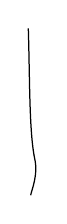
\begin{tikzpicture}[x=1cm,y=1cm]\draw[line width=.45pt] (0,0) .. controls (.02,-.65) and (.01,-1.3) .. (.08,-1.65) .. controls (.13,-1.86) and (.04,-2.06) .. (.03,-2.12);\end{tikzpicture}}

On écrit $F=F_0\amalg G$, et on applique \unsure{lemme|Lemme}

\deleted{\uline{Corollaire 2} Soit $(F_i)_{\unsure{j|i}\in I}$ une famille de composantes connexes deux à deux disjointes. Alors} \deleted{$F=\coprod F_i$} \deleted{la figure engendrée par les $F_i$ est leur somme disjointe $\coprod F_i$} \deleted{et} \deleted{$\subset F$, et si la famille est finie (p. ex. $F$} \deleted{fini} \deleted{figure finie) alors $F=(\coprod F_i)\amalg H$.}

\deleted{Il n'est pas évident que tte figure non vide ait une composante connexe,} \deleted{la difficulté étant dans l'\unsure{existence} \unsure{ou}} \deleted{\unsure{à} des sous-figures \unsure{``compl. dis''|``complém.res''|``comprises''}} \deleted{\inserted{Mais c'est vrai pour les figures de t.f., et a fortiori pour les figures finies. Les}}

\uline{Proposition} Soit $F$ une figure, $A=\overline F\inserted{\subset M}$ l'ens de ses strates. \deleted{Alors l'application} Pour qu'une sous-figure \deleted{$F$} $F_0$ de $F$ soit une comp. conn. de $F$, il f et s que $\overline{F_0}$ soit une composante connexe de l'ens ordonné $A$ (pour l'ordre induit par $\leq$). On trouve ainsi une corr. biunivoque entre l'ens des comp. conn.
